\chapter{Nimble: virtual machine for executing tensor programs}
\label{ch:nimble}

Nimble's instruction set is designed as an abstract machine for executing tensor valued
computations. We can realize this abstract machine by either interpreting it or generating
machine code. This is a tried and true approach utilized by existing languages and languages
runtime such as Java, or C\#.

By lowering the full language to an abstract machine we can reduce it to its core operations,
resulting in a small set of operations we can implement. Our implementation uses a virtual
machine design over an ahead of time compiler. In traditional virtual machines the key
reason to perform ahead of time compilation is to reduce dispatch time, and specialize
away dynamic features such as virtual dispatch.

Due to the design of the Nimble instruction set, instruction dispatch is a very minimal
part of the total runtime, the runtime is defined by kernel execution time.
A virtual machine allows easier experimentation and modification at the cost of dynamically
dispatching instructions, though nothing in our design prevents ahead of time compilation
of the instruction set, but it provides little value for this reason.

For example if we need to produce ahead of time
compiled code, we either must generate calls into a runtime system (which is dynamic),
only removing instruction dispatch, or statically schedule limiting flexibility and
extensibility.

Furthermore our use of TVM means all kernels are ahead of time compiled meaning the
code which dominates execution time, remember most kernels are quadratic or cubic in
complexity, have efficient implementations.

Our extensions for dynamically sized kernels also utilize TVM code generation, enabling
ahead compilation of kernels which perform a form of polymorphic inline caching for shapes,
playing a similar role to what an ahead of time compiler does in traditional JITs.



\subsection{Tensor Virtual Machine}

Although Relay defines an IR and formal semantics
  it does not provide an efficient execution mechanism for the full language.
In the tradition of definitional interpreters we introduced
  a simple interpreter for Relay which implements its formal semantics, which
  we have separately formalized.
Relay’s interpreter can execute the full language but has notable limitations
  that make it unsuited for production deployments.
It is structured as an inefficient interpreter that performs AST traversal to execute the program.
This approach is conceptually simple but inefficient, as the AST traversal heavily relies on indirection.
For example the initial Relay prototype reused the existing ``graph runtime'', to obtain
  acceptable performance for vision tasks.
The graph runtime can only execute simple control-free,
  DAGs of operations.
We can optimize Relay programs and map a subset of them
  to the graph runtime, but any use of new Relay features
  are unsupported.
By introducing models which make use of new features such
  as control flow, recursion, dynamic shapes, and dynamic allocation,
  we must change how execution works.
There are further challenges in compiling dynamic code, such as dynamic scheduling and allocation,
  fully dynamic tensor shapes, and control flow.
The interpreter offers simple solutions for these, but none is sufficiently compelling or optimized.
The simplicity of the graph runtime provides attractive
  properties such as simple serialization, straightforward
  optimal memory layout, and ease of deployment.

To address these challenges we designed a new Relay
  virtual machine.
The Relay virtual machine balances framework the competing approaches to execution,
  providing a dynamic execution environment which can be extended, instrumented, and integrated with other approaches
  like ahead-of-time compilation via a flexible extension mechanism.
The virtual machine is designed to strike a balance between performance and flexibility
  when deploying and executing Relay programs, without giving up the benefits of TVM.
Virtual machine (VM) design is a well-studied area in programming languages and systems,
  and there have been various virtual machine designs for both full-fledged and embedded programing languages.
Previous language VM designs have been heavily tailored to the execution profile of traditional programs.
Traditional programs manipulate small scalar values
  and consist of a large number of low-level instructions.
The sheer quantity of instructions requires instruction execution
  and dispatch to be extremely efficient.
In the context of machine learning we manipulate primarily tensor values,
  using a (relatively) low number of high level instructions.
ML programs’ cost centers are expensive operator invocations,
  such as GEMM or convolution, over a large input.
Due to the execution profile exhibited by ML programs,
  micro-optimizations present in scalar VMs are dramatically less important.

The Relay virtual machine implement a simple register based VM.

The VM consists of three pieces:
\begin{enumerate}
  \item A tensor instruction set for a tensor virtual machine.
  \item A compiler from Relay to the tensor VM.
  \item An implementation of the virtual machine.
\end{enumerate}

\subsection{ISA}
\begin{itemize}
    \item \verb|ret| Returns a value.
    \item \verb|invoke_packed| Invoke a packed function with the specified arguments.
    \item \verb|alloc_tensor| Allocate a tensor of the given size.
    \item \verb|alloc_datatype| Allocate a datatype with the fields.
    \item \verb|alloc_closure| Allocate a closure.
    \item \verb|get_field| Project a field.
    \item \verb|if| Conditional jump based on the condition register.
    \item \verb|get_tagi| Get the object's tag.
    \item \verb|fatal|
    \item \verb|invoke| Invoke a Relay function.
    \item \verb|invoke_closure| Invoke a Relay closure.
    \item \verb|load_const| Load a constant from the constant pool.
    \item \verb|int_const| Store a constant integer in destination.

\end{itemize}
\subsection{VM Compiler}

In order to execute on the VM we wrote a new compiler which
  can lower Relay directly on to the VM bytecode, and then
  executed.
The compiler performs a set of transformations on the high-level
  Relay program before generating code:
\begin{itemize}
  \item A-Normal Form, converts program in to a limited single-assignment form.
  \item Lambda Lift, converts inline functions into top-level definitions,
        ensuring that capture lists are now explicit.
  \item Inline Primitives, ensures that fused functions are inlined into
        the program to enables simplified code generation.
  \item Inliner, general function inlining.
  \item Constant Pool Layout, traverse program collecting all constant values
        and layout them out in memory.
  \item ADT Tag Allocation, allocate the tag assignment for compilation
        to the VM.
\end{itemize}

\subsection{VM}

These three pieces have been completed thus far, we discuss future work in Section
\ref{sec:future}. I plan to submit the entire work to SysML 2020, in early September.


\section{Introduction}
\label{sec:nimble-intro}

As deep learning-based applications have become ubiquitous, so have systems for optimizing, executing, and deploying such applications. A number of systems research projects focus on enhancing the performance of a subset of pre-trained models produced by deep learning (DL) researchers~\citep{Dahl2011taslp, yu2011improved, han2016isca, NIPS2016johnson}.
Specifically, these models represented as static data flow graphs where the sizes of each input and output (i.e. tensors or $n$-dimensional arrays) are known a priori, ensuring the execution path remains unchanged on every invocation.
We refer to models with this static nature as \emph{static models}.
Continued advances in neural networks, especially those in natural language processing, have introduced new dynamism in models, such as control flow \citep{lstm, language_model}, dynamic data structures \citep{tree_lstm, graph_lstm}, and dynamic shapes \citep{devlin2018bert}. We refer to models exhibiting these behaviors as {\em dynamic models}.

As dynamic models mature and continue to move from research to production, it calls for an efficient and cross-platform inference system.
This poses new challenges for deep learning practitioners, as dynamic models introduce input-dependent graph topology, breaking existing system assumptions and invalidating optimizations designed for purely static data flow graphs.
% Dynamic models require an inference system to effectively and efficiently execute across various hardware platforms.
However, no existing solutions fulfill these requirements.

Many existing approaches to dynamic model optimization apply or extend existing deep learning frameworks~\citep{xu2018cavs, gao2018low, yu2018dynamic, jeong2018improving, jeong2019janus, dynet, tf_fold}.
However, deep learning frameworks optimized for training can be limiting in model inference settings due to their rich feature set. In order to realize these features frameworks are often monolithic, large, and non-portable.
%Existing work which builds on frameworks extends the programming model either via sophisticated additions~\citep{yu2018dynamic} or significant runtime overhead~\citep{tf_fold, jeong2019janus}.
%Other work~\citep{xu2018cavs, gao2018low, tf_fold} which is focused on optimizing specific types of models is often hard to generalize to new models, or generalize over all models.
Moreover, approaches which inherit from frameworks rely on third-party kernel libraries such as OpenBLAS~\citep{xianyi2014openblas}, cuDNN~\citep{cudnn}, and MKL-DNN~\citep{mkldnn} to achieve competitive performance. These libraries expose a fixed set of operators for the corresponding hardware, compromising the portability of dynamic models which require a large number of operators with varying data types and shapes. Designing a new interface independent of existing frameworks provides a clean programming model but often at the cost of performance, due to dynamic interpretation of the model~\citep{dynet}.

An alternative approach which has generated significant interest in both academia and industry is the end-to-end optimization of neural networks using deep learning compilers, such as XLA \citep{xla}, Glow \citep{glow}, TVM \citep{tvm_osdi18}, and MLIR \citep{lattner2020mlir}.
Deep learning compilers differ from traditional deep learning frameworks by separating execution into a compilation, and runtime phase. The compilation phase enables whole-model optimization at the graph level, and workload specific kernel code-generation for multiple hardware platforms.

However, deep learning compilers have been primarily restricted to static models due to lack of support for dynamism.
Specifically, in order to compile and execute the dynamic models, a system requires an intermediate representation (IR) which can statically represent dynamic constructs, a code generator
which can generate kernels for dynamically varying data shapes, and a runtime to handle the dynamic execution and kernel dispatch accordingly.
In addition, dynamic-specific optimizations, such as dynamic memory planning, the process of statically optimizing dynamic allocations, are necessary to achieve desirable performance.
None of these features exist in the current deep learning compilers.

To this end, we present Nimble, a high-performance and portable system for compiling, optimizing and executing dynamic neural networks on multiple platforms.
To the best of our knowledge, this is the first attempt to systematically handle dynamic models from a compiler perspective.
First, we introduce type system extensions to handle data with unknown dimension, which is common in dynamic models, by performing type checking and inference for shapes with {\em Any}.
Second, we devise several optimizations specific to dynamic models, including dynamic shape-aware code generation, memory planning, and device placement.
Third, we propose a virtual machine (VM)-based runtime that contains tensor-level operations, enabling the exploration of new runtime and compiler optimizations as well as
being portable, light-weight, and most importantly, able to execute dynamic models.
Experimental results on LSTM~\citep{lstm}, Tree-LSTM~\citep{tree_lstm} and BERT~\citep{devlin2018bert} show that Nimble~lowers the latency by 1.05$\times$ to 19.9$\times$ compared to the best solution whichever on mainstream hardware platforms both in the cloud (Intel CPUs and Nvidia GPUs) and at the edge (ARM CPUs).
%achieves lowest latency over the state-of-the-art solutions and has up to 20.3$\times$ performance speedup on mainstream hardware platforms both in the cloud (Intel CPUs and Nvidia GPUs) and at the edge (ARM CPUs).

In summary, this paper makes the following three core contributions:
\begin{itemize}
    \item Proposes and builds an end-to-end system for efficient dynamic model inference across multiple hardware platforms, including an empirical study to benchmark the results;
    \item Devises several compilation and optimization techniques,
    %for dynamic models,
    including a dynamic type system, a memory planning pass, and heterogeneous device placement mechanism to place computation and data, and a symbolic kernel code generation and shape-based dispatch algorithm;
    \item Designs and implements tensor based abstract machine with a hardware-independent instruction set to efficiently and flexibly execute dynamic models across platforms.
\end{itemize}

The rest of the paper is organized as follows. \autoref{sec:background} reviews the background of dynamic models from the system perspective and \autoref{sec:overview} gives the overview of Nimble.
\autoref{sec:compliation} presents the design and implementation of the compilation flow of Nimble, followed by VM-based runtime in \autoref{sec:runtime}. \autoref{sec:eval} provides the evaluation results using various models on different hardware platforms.
\autoref{sec:relwk} covers related work, and \autoref{sec:conclusion} concludes the paper.

%%%%%%%%%%%%%%%%%%%%%%%%%%%%%%%%%%%%%%%%%%%%% GRAVEYARD

%However, the dynamic nature of these models introduces input-dependent graph topology, breaking existing system assumptions.
%For example, the topology of Tree-LSTM model~\citep{tree_lstm} may change from sentence to sentence depending on its length and structure.
%The input-dependent nature of execution poses new challenges for applying existing inference optimizations to dynamic models.
%Optimizations designed for purely static data flow graphs fail to fully capture model behavior at compile-time.
%Traditionally, researchers modify models by applying workarounds to remove dynamism such as padding to maximum sequence length in order to efficiently execute. However, this may introduce unnecessary computation overhead, and is unable to handle all dynamic cases.

%Deep learning frameworks~\citep{tensorflow, mxnet, pytorch} that are optimized for

%their characteristics significantly simplify their optimization in machine learning frameworks~\citep{tensorflow,mxnet,pytorch} and compilers~\citep{tvm_osdi18,xla,glow}.

%have the following limitations and drawbacks when facing the dynamic model inference scenarios. First, the strength of deep learning frameworks is their rich functionality and optimizations for training and distribution, but often the design choices which optimize for training or distribution introduce challenges for deploying on a variety of platforms.Second, these approaches focus on handling the dynamism of models in the presence of the framework, while purely relying on the framework, and fundamentally, third-party libraries such as OpenBLAS~\citep{xianyi2014openblas}, cuDNN~\citep{cudnn}, and MKL-DNN~\citep{mkldnn} to achieve competitive performance. These libraries only cover a limited set of operators for the corresponding hardware, making it less flexible and portable to support dynamic model inference, which requires to execute a large number of operators with different data types and shapes on various platforms, including high-end server CPUs/GPUs and edge devices. As a result, the framework-based approaches come short in dynamic model inference with less favorable performance and infeasibility to diverse devices.

%Our approach provides three important properties lacking in existing approaches, (1) limited static optimization, (2) high execution overhead, (3) lack of portability and performance portability.
% First the current design assumptions of frameworks input and intermediate representations limit the ability to perform ahead of time optimization. For example TensorFlow's input format is high level, any all though it supports dynamic shapes, it does this via runtime overhead. Its compiler representation XLA only supports kernels which have fixed dimensions.
%when choosing to build a system on top of a framework the set of operators are limited by the underlying capabilities of the framework. For example most frameworks achieve competitive performance by redirecting their operators to carefully hand-crafted and well-tuned kernel libraries that target a few specific hardware architectures with fixed shape and type configurations. These third-party libraries, e.g. OpenBLAS~\citep{xianyi2014openblas}, cuDNN~\citep{cudnn}, and MKL-DNN~\citep{mkldnn}, only contain a limited set of computation-intensive operators for a given hardware platform. These limitations make it challenging to provide simple portability for dynamic models, let alone portable, state-of-the-art performance. As a result, many framework-based approaches have to confine themselves to supporting of a quite limited set of dynamic models for inference, and even when they do execute the performance can be underwhelming.

% \mli{general comments after reading this paper and review feedback. \begin{enumerate}
%     \item should highlight the difference between DL framework and DL compiler, focus on DLC's advantages such as portability, light-weight and performance.
%     \item mention that dynamic NNs are getting popular, while DLC can not deploy these models. This paper will bridge this gap.
%     \item make the system design general, such as these are necessary components to extend any static DLC. By this way we can 1) avoid the feeling that it's just a TVM extension, that will not be accepted by OSDI. 2) make it easy to read so readers don't need to learn TVM and Relay's details
%     \item The design decision of the VM is not straightforward, need to explain why we want to do it. Readers may feel it's an overkill for dynamic NN.
%     \item the performance speedup seems magic. Need to explain the reason which component make it fast
% \end{enumerate}}

% \mycomment{Talk about what are some of techniques to solve the problem and what we do...}
% \mycomment{Meanwhile, we may also want to talk about the difference between our technique and the
%           traditional compiler techniques. Memory management? Granularity of instructions?}

%\item \textbf{Optimization.} Deep learning compilers feature a host of standard compiler optimizations and deep learning specific ones at both graph-level and tensor-level. Most optimizations become non-trivial when dynamism comes into play. Memory planning is among such cases. In dynamic models, as different invocations may go through different paths that need different amounts of memory, we cannot pre-allocate memory as for static models. Furthermore, the shape of input tensors may vary depending on the provided data, i.e. the length of sentences for Tree-LSTM models. Thus, the memory optimization schemes that have worked well for static models are inapplicable to dynamic models.
%For example, operator fusion attempts to combine multiple consecutive operators into a single kernel to eliminate intermediate results, hence reducing costly back-and-forth memory loads and stores. This optimization has been implemented in a variety of deep learning compilers since the input of every operator is known before optimization. However, operator fusion across control flow inevitably complicates the fusion rules as the \texttt{if} and \texttt{else} branches may involve operators that require totally different fusion strategies.

 %Static behavior is most commonly found in image classification models, e.g., VGG~\citep{simonyan2014very}, MobileNet~\citep{howard2017mobilenets}, and ResNet~\citep{he2016deep}.
%For example, memory could be allocated before runtime and schedules could be confined to a relatively small set of parameters for each operation as the execution path is fixed for arbitrary input in the static scenario.

%primarily come from deep learning frameworks~\citep{tensorflow, mxnet, pytorch} and runtime systems~\citep{xu2018cavs, gao2018low}.
%For example, Tensorflow Fold \citep{tensorflowfold}

%%%%%%%%%%%%%%%%%%%%%%%%%%%%%%%%%%%%%%%%%%%
% old intro

% There are two clear levels to support full dynamism, dynamism introduced by the frontend language
% such as found in PyTorch and other expressive dynamic neural network frameworks. The second level of
% dynamism is innate to models, take for example a model which dynamically produces the inputs for an
% inner RNN.

% Frameworks such as PyTorch, and JAX have begun to address the first challenge by employing
% techniques from JIT compilation to find traces of user programs with stable properties (e.g., tensor
% shapes). After obtaining a stable trace the framework must produce an efficient implementation for
% the static fragment. Even if we eliminate behaviors like conditionally construction of the model
% based on whether it is executed in training or inference mode, true dynamism remains. For example
% BERT uses dynamic behavior which generates runtime dependent sized tensors. TODO CHECK THIS.

% Existing state-of-the-art optimizing compilers for deep learning provide limited support for
% efficiently compiling these type of operations. In particular the ability to quickly prototype new
% execution or compilation strategies is challenging.

% In this work we introduce Nimble an extension to TVM's Relay IR which provides efficient
% compilation and execution of neural networks using data structures, control-flow, closures and
% dynamically sized tensors.

% Old contributions:
% \begin{itemize}
%     \item An extension to the type system of Relay to support dynamic dimensions.
%     \item A new efficient runtime system and virtual machine for Relay programs.
%     \item A framework for exploring code generation strategies.
%     \item A set of optimizations to improve code generation.
% \end{itemize}

\section{A System Perspective to Dynamism}
\label{sec:nimble-background}

%This section briefly discusses two representative classes of DL models: static models and dynamic models. We also explains the challenges in performing models inference for dynamic models which motivates the design of Nimble.

Dynamism is now common in state-of-the-art deep learning models in various forms, i.e. control flow, data-dependent model architecture, and variable data shapes imposed by dynamic batch size and/or input length.
In the presence of these features, it becomes impossible to pre-compute certain program properties ahead of time, hence only a limited subset of optimizations available for static models can be directly reused.
In this section, we first review the existing systems to support dynamism, followed by the discussion of supporting dynamic models using deep learning compilation techniques. Based on the observation, we propose our system Nimble and give an overview of it.

\subsection{Existing systems}
\label{sec:background:existing}
Researchers working on dynamic models typically use flexible deep learning frameworks to build proof of concept models, and then attempt to optimize the model using the builtin capabilities of the framework when deploying at scale.

Deep learning frameworks describe the model in either an imperative (define-by-run) or symbolic (define-then-run) fashion.
Imperative frameworks, such as DyNet~\citep{dynet} and PyTorch~\citep{pytorch}, although user friendly and flexible, may reduce performance due to eagerly executing each computation in isolation.
Both DyNet and PyTorch support executing compute-intensive operators by reusing high-performance implementations from vendor libraries, however, the inherent nature of imperative execution substantially limits optimization, i.e. no operator fusion and batching.
In addition each execution path requires the creation of a path specialized static data flow graph introducing overhead in dynamic cases, which can sometimes be unacceptable for particular application.

Not only do frameworks rely on vendor provided libraries, but many are written in a combination of multiple programming languages such as C++ and Python. The inclusion of platform specific libraries and/or arbitrary Python program fragments limits deployment and retargeting.
Platforms such as resource limited edge or embedded devices do not support these libraries and/or languages limiting these solutions from executing on some platforms without serious re-engineering, leading to solutions such as TensorFlow Lite.
Imperative programs are extremely effective at helping researchers prototype and test preliminary ideas, but not an ideal or systematic solution to deploying dynamic models at scale.

Alternatively, other deep learning frameworks use a symbolic approach, in which a user specifies the program as a data structure which can later be optimized, deployed, and executed. Frameworks in this style such as TensorFlow and MXNet already have introduced support for dynamism, such as control flow and dynamic batching~\citep{yu2018dynamic, tf_fold, mxnet-control}. Although these make it possible to use dynamic features, the extensions add complexity to an already complex programming model, and are often less integrated into the framework, requiring users to use a sophisticated modified programming model when defining dynamic models.

In addition, in some cases, it is possible to reduce the dynamic model to a static one. For example, in RNN models with variable input length, a maximal input length can be used to statically unroll the network, and padding applied to the inputs in order to directly adopt optimizations performed on static models~\citep{zhang2018deepcpu}. However, transforming a dynamic model into a static one for optimization is inflexible and only works for a subset of dynamic models. Programmability and flexibility aside, the above solutions inherit the cumbersome codebase of the deep learning frameworks which have poor portability to multiple platforms, especially edge devices. From a systems perspective, they are too heavy-weight to be adopted in these cases.

In order to enjoy the flexible description of dynamic models provided by high-level frameworks and the performance advantages of ahead of time optimization, prior work like Janus~\citep{jeong2019janus} attempted to bridge these two programming models for dynamic models.
Janus was implemented as an extension to TensorFlow which parses the model defined in TF Eager and use speculative execution to eliminate control flow constructs within the model.
Although this solution provides good performance in a subset of cases, it suffers from performance loss when speculative assumption is violated.
%\yida{@Haichen, we may also discuss the usage of ? here. Or we can defer the discussion of ? to section 3.}
Also, as it is still based on the framework, this solution inherits the drawbacks of poor portability.

Specific runtime systems were recently proposed to handle dynamic models~\citep{xu2018cavs, gao2018low}. These systems are designed to address system-level issues that plague framework-based approaches, e.g., large overhead introduced by data flow graph construction.
However, other issues, such as software dependencies, remain, which makes these runtime systems not standalone, but a customized component of a larger deep learning framework.

\subsection{Limitation of Deep Learning Compilers}
\label{sec:background:dlc}
As discussed in~\ref{sec:background:existing}, existing solutions to dynamic models have various limitations, the most pressing of which is the lack of portability and cross-platform support.
A generic system which handles dynamic models for efficient inference is missing.
Conceptually, this system should handle all dynamic models, provide portable performance across multiple platforms, and execute everywhere by virtue of being light-weight and dependency-free.
With these goals in mind, deep learning compilers are a promising direction to explore, as these techniques aim to perform end-to-end optimization on models that can run with minimal memory footprint over multiple platforms.


% \begin{figure}[t]
%   \centering
%   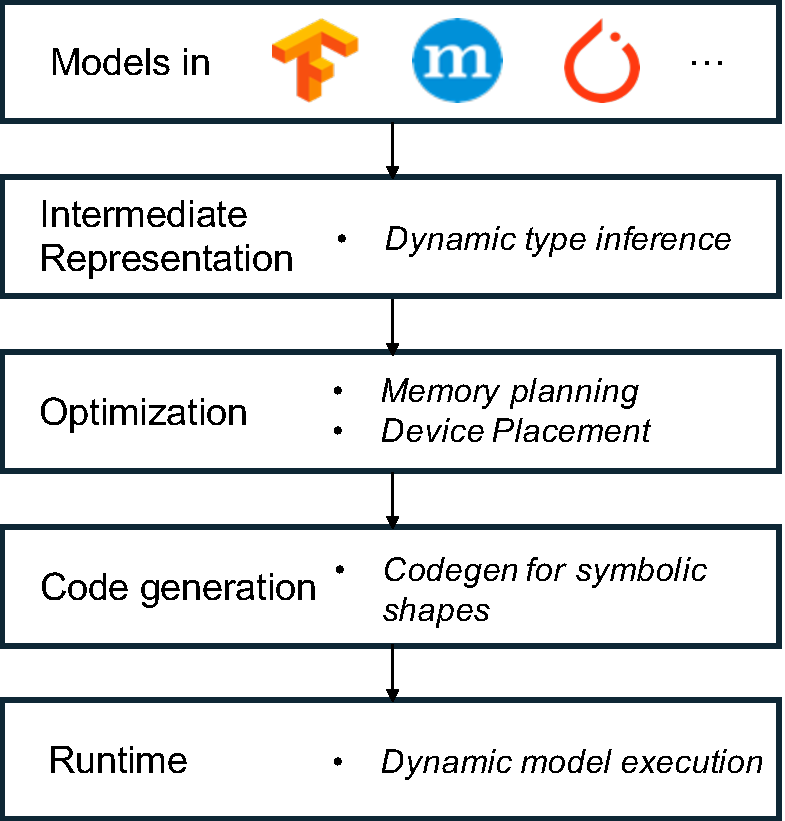
\includegraphics[width=.7\linewidth]{figs/dlc.pdf}
%   \captionof{figure}{
%   %\protect\yida{Can delete this figure if running out of space.}
%   A generic deep learning compiler workflow in multiple stages. Existing deep learning compilers are unable to process dynamic models due to lacking of the functionalities listed in each stage.}
%   \label{fig:dlc}
% \end{figure}

However, current deep learning compilers are not able to process dynamic models due to missing the following dynamism-specific features.% in the \emph{type system}, \emph{codegen}, and \emph{runtime}, along with dynamism-oriented optimizations such as \emph{memory planning} and \textit{heterogeneous device placement}.

\begin{itemize}
\item \textbf{An IR for representing dynamism.} Performing data type and shape inference on static models is straightforward as both the data type and shape of each operator are known during declaration and remain unchanged during runtime. However, the shape of an input tensor may vary wildly across different input samples in a dynamic model. The emergence of control flow constructs further complicates this problem as different execution paths can emit substantially different data. A fully static IR, hence, is inadequate to cope with the dynamic characteristics of these models.

\item \textbf{A set of dynamic-oriented optimizations.} Existing deep learning compilers, e.g. TVM \citep{tvm_osdi18} and Glow \citep{glow}, expect static input for each optimization. The memory size of each tensor is pre-allocated and their live cycles are determined using a dedicated optimization pass. They also ensure the homogeneous execution of the entire model because all kernels are executed on the same device with no data transfer between the host and device after a kernel is launched. However, these optimizations may completely break when dynamism appears. Now different execution path possibly requires different amount of memory and the sizes are not available before runtime. Certain simple IR nodes may also be introduced to help runtime type inference and memory allocation. The operations in these nodes are intrinsically more CPU friendly, which would lead to the serious performance problem if not placed on the correct device.

\item \textbf{A symbolic kernel code generator.}
Code generation (codegen) is responsible for generating high-performance executable kernels for operators. Recent research \citep{tvm_osdi18, glow, chen2018learning, zheng2020flextensor, adams2019learning} has achieved impressive results in kernel performance with static shapes on multiple backends.
Nonetheless, challenges in codegen with symbolic shapes remain unexplored.
After applying the same set of loop optimization, kernels generated with symbolic shapes could still perform bad if the loop boundary is not handled properly.
Meanwhile, kernel tuning under symbolic shape settings become more challenging as the search space grows exponentially.

%\yida{@Haichen, please revise this part accordingly. I feel that we should talk about about symbolic. And perhaps make it shorter, comparable with the other two points}
% The same operator (e.g. convolution) with different data shapes may require different kernels with different execution schedules to obtain preferable performance. There is no ``one-size-fits-all'' kernel and/or schedule that delivers consistently ``the-best'' performance across invocations with vastly different data shapes in a dynamic model. Instead, it requires the code generator to take the varied shapes into consideration and possibly generate a family of specialized kernels to maximize the performance of a dynamic operation. In addition, some common operators are well-optimized on specific platforms (e.g. MKL-DNN for Intel CPU and CuBlas for Nvidia GPU), and the code generator should be able to select kernels from third-party libraries if they will achieve the best end-to-end performance.

\item \textbf{A light-weight and cross-platform runtime.} For efficiency purpose, the runtime of static models could be simply designed a sequential executor that traverses the input data flow graph in the topological order and invokes operators sequentially. However, the execution path of dynamic models can only be determined at runtime and the kernels for certain operators must be dispatched according to the data shape determined at runtime, making a simple graph-style runtime insufficient.
\end{itemize}

Figure~\ref{fig:dlc} summarizes a generic deep learning compiler workflow in multiple stages, with the missing parts to supporting dynamism listed in each stage.  %\zhicomment{Figure needs to be updated, add heterogeneous device placement to optimization}.

\section{System Overview}
\label{sec:nimble-overview}

% \begin{figure}[t]
%   \centering
%   \includegraphics[width=\linewidth]{figs/nimble.pdf}
%   \captionof{figure}{Nimble overview. Nimble consists of a compiler that handles model with dynamism and a runtime that executes dynamic models in multiple platforms. Both components have multiple modules, which will be introduced in detail in the corresponding sections.}
%   \label{fig:vm}
% \end{figure}

After reviewing systems for dynamic deep learning models, this section gives an overview of Nimble, a high-performance and flexible system for compiling and optimizing dynamic models for multiple platforms. In general, the design goals of Nimble are:
\begin{enumerate}[leftmargin=*]
    \itemsep 0em
    \item {\bf Supporting dynamic models.} Nimble targets models with all types of dynamism, including control flow, dynamic data structures and varied data shapes.
    \item {\bf Being portable and light-weight.} The module that Nimble produces should be executable across a number of platforms on the cloud (high-end CPUs and GPUs) and at the edge (low-power CPUs and GPUs). The runtime should be light enough to run on devices with minimal compute power and memory capacity.
    \item {\bf Enabling high performance.} Nimble should be performant in the context of dynamism across platforms.
\end{enumerate}

Figure~\ref{fig:vm} shows the system architecture of Nimble that we propose to achieve the aforementioned design goals.
It is a system consisting of two major components, namely a compiler and a runtime.
Nimble takes a model in the format of mainstream deep learning frameworks, converts it into a unified intermediate representation (\textit{IR}), then optimizes and compiles the IR into an executable that contains both platform-agnostic bytecode and platform-dependent kernel code, and finally loads the executable to execute in the VM-based runtime.
%\yida{The VM high-level description may be moved to the next paragraph, after compiler high-level description.}
%The bytecode is designed to only express the semantics of the IR, e.g. the control-flow and platform-dependent kernel invocation, through dedicated instructions, which contributes a negligible portion of the total execution time, as we will show in~\autoref{sec:eval}.
The bytecode is executed by Nimble's runtime interpreter, which is shareable across various platforms.
This design effectively enables us to only maintain one version of the execution logic, but focus more on the performance critical operator kernels.
The kernels are highly-optimized for a specific hardware platform to achieve high performance.
%Kernels optimized for data with different shapes are compiled separately and dispatched accordingly.

To effectively support dynamic models without performance degradation for static models, we introduced various analysis and optimization techniques in Nimble's compiler.
First, a set of IR extensions are devised to represent dynamic shapes (\textit{Any} shape) and dynamic allocations for static optimization of dynamic program behaviors (\autoref{sec:compliation:typing}).
Second, shape functions are attached to operators to compute the output shapes dynamically and perform type checking at runtime (\autoref{sec:compilation:shape-func}).
Third, a memory planning optimization is employed to reduce amount of memory consumed (\autoref{sec:compliation:memory}).
Fourth, a heterogeneous device placement mechanism is designed to place IR nodes on ``the-best'' device to reduce expensive cross-device data transferring and synchronization (\autoref{sec:compliation:hetero}).
Finally, the compiler features a code generator that is capable of specializing the code generation of certain likely shapes (\autoref{sec:compliation:codegen}). Once the executable with dynamic behavior is compiled, the VM-based runtime can load and interpret it with intelligent dynamic kernel dispatching (\autoref{sec:runtime}). We detail the design and implementation of each of these features in the followed sections.

\section{Compiler Support for Dynamism}
\label{sec:nimble-compliation}

A key challenge preventing existing deep learning compilers from handling dynamism is the lack of a uniform and dynamic representation. For example, optimizations and runtime of existing IR, e.g. TVM \citep{tvm_osdi18}, assume the presence of static shape information in numerous places. These assumptions are present in many other so-called graph compilers and introduce quite a few challenges for optimization.

In order to handle dynamism, we design a set of IR extensions which expose the essential semantics required to optimize dynamic programs. The approach is implemented in Nimble on top of the Apache TVM (version 0.6) deep learning compiler infrastructure \citep{tvm_osdi18} to leverage its frontend converters from various DL frameworks to its IR. TVM's frontends alleviate the need to frontend specific details enabling our work to focus on contributions such as IR extensions and optmizations. To use Nimble, one only needs to feed it with a pre-trained model, perform compilation and then inference. Furthermore, the lessons
here are applicable to other compiler efforts such as TensorFlow's MLIR support or PyTorch's TorchScript and TensorExpr (a Halide and TVM inspired DSL for kernel codegen) work. The below section
describes how we transform standard TVM programs into a our dynamic dialect which enables us to easily apply static optimizations to dynamic programs, much as we do in traditional compiler optimization.

In this section, we detail three key components required to compile dynamic models.

\begin{itemize}
    \item An extended type system which enables statically tracking dynamic shapes.
    \item A series of optimization passes that make dynamic output shapes, allocation, and device placement explicit.
    \item A set of codegen techniques for producing code for kernels with dynamic input and output shapes.
\end{itemize}

\subsection{Typing}
\label{sec:compliation:typing}
Deep learning compilers use type systems to represent, check and infer the data types and shapes of tensors. In some frameworks and compilers this is separated into two steps, shape inference and data type inference. TVM~\citep{roesch2019relay} performs both simultaneously and refer to them as type inference, terminology we will use throughout the section.

A {\em Tensor Type} is designated by an $n$-dimensional shape (defined as a tuple of integers describing the tensor's dimensions) and a data type (e.g. \texttt{float32} or \texttt{int64}).
Current deep learning IRs only support codegen when all dimensions of a tensor's shape are known at compile-time.
Static shapes are mandatory for type inference and checking in existing deep learning compilers.

In the context of dynamic models, many data shapes can only be determined at runtime. Therefore, the previous assumption of static data shapes does not hold.
In order to support dynamic data shapes, Nimble introduces a special dimension called Any~to represent statically unknown dimensions.
For example, we can represent a tensor type as \texttt{Tensor[(1, 10, Any), float32]},
where the size of the third dimension in this tensor is unknown while the other
two dimensions have concrete values.
This concept is relatively uncontroversial, and has been introduced in other frameworks.
Janus \citep{jeong2019janus} uses similar denotation to represent a dynamic dimension but only for type unification, while Nimble extends type inference to handle Any~as described next. We do not support tensor types with dynamic ranks given the relatively limited use cases and optimization opportunities.
%\yida{Do we need the following sentence?}The challenge of introducing a dynamic shape extension is adapting each layer of the system to handle it in a way that does not greatly degrade performance.

\noindent
{\bf Operator Type Relation} A type relation describes the relationship between the types of operator inputs and outputs. The type system of TVM's Relay IR relies on these type relations to infer and bidirectionally propagate type and shape relationships between inputs and outputs of operators across the whole program.
For example, the type relation for broadcasting operators (e.g. \texttt{broadcast\_add}) performs the shape calculation following the NumPy broadcasting rules\footnote{\url{https://docs.scipy.org/doc/numpy/user/basics.broadcasting.html}}.

The type relation must be generalized to properly handle dynamic shapes. For example, a program which grows a tensor on each loop iteration (a case existing in the decoder of many NLP models) is both impossible to type and compile without proper type system support. With the introduction of Any, we are able to improve the existing type relations to support dynamic models.

There are two cases that must be handled after we introduce Any~to the type relations.
First, operators such as {\tt arange}\footnote{{\tt arange} generates a range of values in a (start, stop, step) interval the arrays output size is a function of input arguments.} and {\tt unique}\footnote{{\tt unique} selects the unique elements of a tensor.} have dynamic output shapes depending on the input data, which will be described in Any.
% We can now describe the type relation using the enhanced type relation functions with Any but not before.
% For example, type relation of {\tt arange} can be expressed as follows
% \[
% arange: fn(start: fp32, stop: fp32, step: fp32) \rightarrow \langle [Any], fp32 \rangle
% \]
Second, when input shapes of a type relation contain Any~dimension, the type relation needs to propagate Any~correctly to the output types and relax typing constraints that hold in the static cases when necessary.
%For example, type relation for {\tt broadcasting} operators determines the compatibility between corresponding dimensions from both inputs if they are equal or one of them is 1 according to the Numpy broadcasting rule.
For example, the rules
for broadcast type relation given the matching dimension from two inputs when having Any~are defined as follows:
\begin{align*}
  \textrm{broadcast\_rel}(Any, 1) &\rightarrow Any \\
  \textrm{broadcast\_rel}(Any, d) &\rightarrow d ~~~~~~(d > 1) \\
  \textrm{broadcast\_rel}(Any, Any) &\rightarrow Any.
\end{align*}
Note that due the presence of dynamic shapes these type relation rules can no longer rule out all type errors at compile-time.
For example, for the second rule shown above, when Any~is neither 1 nor $d$ at runtime, it then violates the broadcast type constraints.
To address this, we take the gradual typing~\citep{gradualtyping} approach and leave certain type checking at runtime after Any~is instantiated by a
concrete value (see \autoref{sec:compilation:shape-func} for more details).
One could eliminate these errors using a more advanced type system, but at increased complexity.

\noindent
{\bf Type Inference} One caveat of the Any~dimension is that unknown dimensions will propagate during type inference, reducing chances for shape specialization.
For example, if we use an operator such as {\tt arange} to produce a tensor with dynamic shape (i.e., \texttt{Tensor[(Any,), f32]}) and later {\tt broadcast\_add} to a tensor with static shape (i.e., \texttt{Tensor[(5, 1), f32]}), the output shape will also contain an Any~dimension (i.e., \texttt{Tensor[(5, Any), f32])}.

To limit the contamination of Any, we further introduce {\em sub-shaping} to improve the precision of types computed by type-inference.
Much like sub-typing used in popular programming languages \citep{LiskovTPLS1994,AmadioAmadioTPLS1993}, our extension enables values with more specific shape information to be passed in contexts which require less specific shapes.
Further, we perform extra analysis on each Any~dimension to detect if two Any~dimensions point to an identically sized dimension. We can use this analysis in the downstream compilation to generate shape-specialized code during codegen.
% We treat concrete dimension and symbolic dimension as a sub-shape of Any.
% \yida{The following sentence is problematic with grammatical error. We need to explicitly define what is an argument.}Rules for invoking a function, suppose fn type is $fn\langle T_1, \dots, T_n\rangle$,
% and arguments are $T'_1, \dots, T'_n$, the rules are defined as follows
% \begin{align*}
%   \textrm{union}(T_i, T'_i) &\rightarrow T_i \\
%   \textrm{join}(T_i, T'_i) &\rightarrow T'_i
% \end{align*}

\subsection{Shape Function}
\label{sec:compilation:shape-func}
%Existing deep learning compilers only deal with static shapes, enabling all shape computation to occur at compile-time.
%Therefore, it is easy to allocate memory for the tensors using static shape information to compute the precise amount of storage needed for each tensor.
%However, introducing Any~invalidates this pre-allocation mechanism as the tensors may now contain dynamic dimensions.
The introduction of Any~dimension invalidates the pre-allocation mechanism adopted in the existing deep learning compiler.
Instead, we now have to track the amount of memory required to be allocated in parallel to computing.
Furthermore, static type checking cannot eliminate all type errors at compile-time due to dynamic tensor shapes.
Consequently, we define a {\em shape function} to compute the output shape for storage allocation and verify the type relation in accord with the semantics of every operators.
The shape function is similar in structure to the type relations described in \autoref{sec:compliation:typing} but are present at runtime instead of compile-time.
The shape function enables compiling and embedding the computation of output shapes into the program.

According to the characteristics of the operator, we divide the shape functions in three different modes: data independent, data dependent, and upper bound.
{\em Data independent} shape functions are used for operators in which the output shape only depends on the shapes of inputs such as normal 2-D convolution.
{\em Data dependent} shape functions require the concrete input values to compute the output shapes. For example, the output shape of \texttt{arange} depends on the value of start, stop, and step.
In addition, there are certain operators such as Non Maximum Suppression (\texttt{nms}) where the complexity of computing the output shapes is on par with the complexity of executing the operator itself.
In order to avoid the redundant computation, we use an {\em upper bound} shape function to quickly estimate an upper bound shape for the output.
We also require such operators to return the output shape along with output value, so as to use the real shape to slice the output tensors into precise output shape and layout.

It is worth noting that in the presence of dynamic shape functions, operator fusion needs to be specially taken care of.
Operator fusion, which combines {\em basic operators} into a {\em composite operator}, is a critical technique for performance optimization as it reduces unnecessary memory copies and improves the cache locality.
%However, we only define the shape function at elementary operator level. As a result, we also must fuse shape functions in parallel with the operator fusion.
The compiler can easily connect the shape functions of basic operators to form the shape function for a composite operator when all shape functions are data independent.
However, a basic operator with a data dependent or upper bound shape function cannot be fused to other operators, i.e., taking the outputs of other operators as its inputs to fuse together, as the shape function requires to access to the intermediate result within a composite operator.
As a result, we explicitly define the fusion policy to prevent this from happening.
%If all basic ops in a composite op have data independent shape functions, it is straightforward to generate shape function for this composite op as we can just connect the shape functions of basic ops together. However, a composite op is invalid if a basic op that has a data dependent or upper bound shape function takes the intermediate output of another basic op as input.
%Because the intermediate result in a composite op is inaccessible from outside, the data dependent shape function cannot collect all arguments it required. Thus, we revise the operator fusion policy correspondingly to make sure composite ops generated by the operator fusion pass will be valid.

%Due to our definition of shape functions we are able to perform fusion using a generalized version of the algorithm used for standard operator fusion which handles passing the appropriate input shape or input depending on the shape function. For example imagine that the fuse operator has a single input that was originally used an operator that requires the input, and the second fused operator requires the input shape. Depending on the type of the shape function defined above, we handle operator fusion in the following manner. Any data independent shape functions could be fused with other operators. Any fused group can only have at most one shape function and it should be fused together with the operator that needs shape function.

\subsection{Memory Planning}
\label{sec:compliation:memory}
Deep learning workloads are dominated by two key aspects, compute-intensive kernels and memory allocation. Many deep learning compilers use a form of static memory planning which tries to coalesce memory and minimize allocations. For devices such as GPUs these optimizations are essential for reducing memory fragmentation and ensuring allocation does not hamper kernel performance. Existing deep learning compiler IRs hide memory allocation behind a functional interface, where each operator implicitly allocates their output storage. Then before execution, the system performs static-memory planning on the data-flow graph enabling efficient pre-allocation of the required memory. Due to this ``out-of-band'' nature of memory allocation, it is challenging to customize, modify or compose memory optimizations with other passes. For example, if one needs to adjust memory allocation for heterogeneous execution, modifications to the runtime are required.

Alternatively, some systems lower the entire program to low-level IRs such as LLVM~\citep{llvm} in order to perform optimizations. Due to the coarse-grained memory semantics of deep learning models, it is essential that memory optimizations occur at a suitably high-level of abstraction before essential program facts are lost. Moreover, as discussed in~\autoref{sec:compilation:shape-func}, we have introduced new ways to account for the handling of dynamic allocations, which further complicate memory analysis.
In order to perform dynamic memory planning we have extended TVM's Relay IR, using these extensions we translate a IR dialect where all memory allocations are implicit to one where buffers are allocated and passed around explicitly. The key to this transformation is an inter-procedural change of calling convention, with each operator now taking its outputs explicitly it is possible to track and transform allocations.
In particular, we have introduced four new IR constructs, (a) \verb|invoke_mut(op, inputs, outputs)| which takes outputs as mutable in-out arguments, (b) \texttt{alloc\_storage(size, alignment, device)} which allocates a region of memory of a particular size, (c) \texttt{alloc\_tensor(storage, offset, shape, dtype, attrs)} which allocates a tensor at a particular strorage offset with a shape and data type, and (d) \verb|kill(tensor)| which frees a tensor before its reference count becomes zero due to exiting the frame. Note that in the below code examples \texttt{Tensor<d1, ..., dn>} is shorthand for a tensor of shape \texttt{(d1, ..., dn)} containing floating point values.

We can demonstrate how to transform a single statically shaped operation such as broadcasting addition.

%\begin{Verbatim}[fontsize=\small]
\begin{lstlisting}
fn main() -> Tensor<10> {
  let t1, t2 : Tensor<10> = ...;
  add(t1, t2)
}
\end{lstlisting}
%\end{Verbatim}

Here we only must allocate a single buffer, the return buffer for the addition operation.

%\begin{Verbatim}[fontsize=\small]
\begin{lstlisting}
fn main() -> Tensor<10> {
  let t1 = ...; let t2 = ...;
  let storage = alloc_storage(40, 64, cpu(0));
  let out1= alloc_tensor(storage, 0, (10), f32);
  invoke_mut(add, (t1, t2), (out1));
  out1
}
\end{lstlisting}
%\end{Verbatim}

The above transformation replaces all operator invocations with a call to \verb|invoke_mut| allocating storage
for backing a single tensor from allocated at offset zero.
The key insight is to internalize a notion of memory allocation into the IR, enabling static optimization of
both static and dynamic allocations presence of control and dynamic shapes. We realize our shape functions as fragments of TVM's tensor expression language which computes the output shape for a particular operator. As detailed in~\autoref{sec:compilation:shape-func} our shape functions may require the input, the input \textit{shape}, or both.
Our uniform treatment of shape functions as standard tensor expressions enables them to be fused and optimized like normal, but one challenge is that we must now manifest allocations in a fixed point until we allocate for both the compute and necessary shape functions. We illustrate this below with a single dynamic concatenation.

%\begin{Verbatim}[fontsize=\small]
\begin{lstlisting}
fn (x: Tensor<?,2>, y: Tensor<1,2>)->Tensor<?,2> {
  concat((%x, %y))
}
\end{lstlisting}
%\end{Verbatim}

This is the same transformation as the previous example with the addition of carefully inserting
invocations to the shape function to compute output buffers sizes for the dynamically sized kernel.

%\begin{Verbatim}[fontsize=\small]
\begin{lstlisting}
fn (x: Tensor<?,2>, y: Tensor<1,2>)->Tensor<?,2> {
  let in_sh0 = shape_of(x);
  let in_sh1 = shape_of(y);
  let storage_0 = alloc_storage(16, 64, ...);
  let out_sh0 = alloc_tensor(storage_0, ...);
  invoke_shape_func(concat,
      (in_sh0, in_sh1), (out_sh0,), ...);
  let storage_01 = alloc_storage(...);
  let out_0 = alloc_tensor(
      storage_01, shape_func_out_0, ...);
  invoke_mut(concat, (x, y), (out_0));
  out_0
}
\end{lstlisting}
%\end{Verbatim}

After the transformation you may notice we have introduced calls to \verb|shape_func| which invokes a shape function for a kernel. The shape function requires input shapes as arguments which further require us to invoke \verb|shape_of| for both \verb|%x| and \verb|%y|. \verb|shape_of| will be directly mapped to a VM instruction to retrieve the shape of a tensor at runtime. More description of it will be provided in \autoref{sec:compliation:hetero}.

Now that the all allocations are explicit in the IR we can provide analogous optimizations in the static
case on dynamic programs, for example we have implemented a storage coalescing pass which groups storage
into a larger region which we can then multiplex tensor allocations on to.


\subsection{Heterogeneous Device Placement}
\label{sec:compliation:hetero}
As discussed in Section \autoref{sec:compilation:shape-func}, shape functions are executed at runtime to calculate the output shape of an operator. These functions must execute on the CPU due to the host-interaction model of GPU like devices. In the case of heterogeneous execution (i.e., CPU and GPU) it is essential to carefully schedule the execution of shape functions and kernels as improper scheduling can be disastrous for performance. For instance, considerable overhead will occur if inputs to shape functions must be copied from GPU due to the cost of data transfers and synchronization. To minimize the performance penalty, we analyze the program allocations to place sub-expressions on the most suitable devices.

We introduce a unification based analysis for computing the correct device placement and allocation based on the previous scheduling of the compute kernels. The goal of our device analysis is assigning each IR node in a way that minimizes the number of cross-device copies. We introduce a concept of \texttt{DeviceDomain} to represent the domain of a device, including source and destination. Each expression in the IR defaults to the empty domain, meaning there are no constraints on its device placement. In addition, two new IR constructs are introduced to facilitate the heterogeneous execution of VM, namely \verb|device_copy| and \verb|shape_of|. The former performs a data transfer between different devices and is inserted when a cross-device data copy is mandatory. The latter is used to retrieve the shape of a tensor at runtime and is used to efficiently compute the input shapes for shape functions. Our analysis is formulated as a set of device placement rules which describe how device constraints flow, and then we use unification, a technique common in type inference and compilers in order to compute precise device placement.

\begin{itemize}
    \item \verb|shape_of|. Defaults to the CPU domain because we can access a Tensor's shape regardless of which device it is placed on.
    \item Shape functions. These IRs take the output of one or multiple \verb|shape_of| and then derive the shape of an operation according to predefined type inference rules. The output of a shape function is used to compute the amount of memory that this operator requires at runtime, which only needs a few cheap scalar arithmetic computation. Therefore, the inputs and outputs would be better on a CPU domain as well.
    \item \verb|device_copy|. The input and output of this IR are on different domains as it copies data from one domain to another. The device domains of the input and output are propagated in the opposite directions to other IR nodes that are reachable to/from the device copy node.
    \item Memory operations. The device domain of storage from \verb|alloc_storage| is designated in the expression, and later is propagated to the device domain of the tensors allocated from this storage via \verb|alloc_tensor|.
    %in the instruction computation of the allocation size and the shape for memory operations, such as \verb|alloc_storage| and \verb|alloc_tensor|, should be on CPU due to low computation intensity.
    \item \verb|invoke_mut|. All arguments used in the \verb|invoke_mut| must have the same device domain.
    \item Other common IR nodes. The device domain of other common IR nodes, e.g. variables, constants, operators, etc., can be directly propagated from the above nodes.
\end{itemize}

Based on the rules defined above, we use a union-find data structure to bidirectionally propagate and unify the device placement of each IR node. We introduce two operations, \texttt{union(s, t)} and \texttt{find(s)}, to achieve \texttt{DeviceDomain} unification throughout the entire program. \texttt{union(s,t)} unions the equivalence device domains of \texttt{s} and \texttt{t} into one equivalence domain when the device types match. \texttt{find(s)} returns the representative of the device domain that \texttt{s} belongs to. These two operations are applied until all IR nodes are annotated. The result of the heterogeneous device placement composes with memory planning and shape function insertion resulting in correctly placed allocations.

\subsection{Symbolic Codegen}
\label{sec:compliation:codegen}
%\yida{Should we mention the mechanism of invoking third-party libraries in this subsection?}
Deep learning compilers~\citep{tvm_osdi18, halide} have demonstrated competitive performance compared to manually tuned kernels on multiple platforms. Recent trends apply machine learning based search to further reduce or eliminate complex manual performance tuning, existing work applies both template based~\citep{chen2018learning, zheng2020flextensor} and beam search based~\citep{adams2019learning} ones.

However existing work which focuses on tuning in the presence of static shapes falls short with symbolic or dynamic shapes. There are two inherent challenges with regard to codegen with symbolic shapes.
\begin{itemize}
    \itemsep 0em
    \item How to achieve the same performance of kernels generated with symbolic shapes as that with static shapes when applying the same schedule?
    \item How to extend the machine learning based approach to tune kernels with symbolic shapes?
\end{itemize}

Loop parallelism and loop tiling are common optimization techniques that exploit multi-core capabilities by achieving data access patterns which are memory hierarchy aware for both CPUs and GPUs. However, the combination of these techniques lead to complex loop boundary conditions. In many static cases, it is possible to prove these conditions always hold, and thus eliminate checks which hamper further optimizations such as unrolling.
While straightforward to handle with static shapes, it becomes a non-trivial challenge when performing symbolic codegen. If not carefully handled, the boundary condition checks will stay, leading to poor performance.

To address this issue, we generate multiple kernels according to the residues modulo of the tiling factor and then dispatch based on the actual shape at runtime.
For example, suppose a symbolic dimension $x$ is divided by a factor of 8, we then duplicate the generated kernel for 8 times, and replace the symbolic var $x$ by $8k+r$ in each copy, where $k = \lfloor x / 8 \rfloor$ and $r \in [0..7]$. By applying this technique in conjunction with an enhanced symbolic expression simplification pass, we can eliminate most boundary checks to achieve performance that is nearly identical to kernels compiled with a single static shape. Lastly, we automatically generate a dispatch function that invokes the corresponding kernel based on the residue.
%because this function is also generated in the IR we can compile and optimize it like other code ahead of time.
In addition, the dispatch function can be extended to invoke either compiler generated kernels or third party library whichever is faster from the profiling results.
The increased kernel size is relatively small compared to the overall deep learning models.
In extreme cases where resources are extremely limited, we can either generate fewer number of kernels than the tiling factor or reduce the tiling factor to find an acceptable trade-off between code size and performance.

A known issue to machine learning based tuning is that it may take a long time (usually hours) to find the best schedule for a single kernel. When it comes to symbolic shapes, the tuning time may be exponentially longer if we naively tune for every possible shape. In this paper, we extend the template based tuning approach for symbolic shapes in order to make tuning time tractable. The template based tuning approach takes a human-defined code template and a search space, and searches the best configure within the search space by using machine learning algorithms.
%by building on the techniques explored in based~\citep{chen2018learning}.
We observe that a good configuration for one shape usually performs well on other shapes. Based on this observation, we devise the following mechanism to tune the kernel for symbolic shapes.

\begin{enumerate}[leftmargin=*]
    \itemsep 0em
    \item First replace the symbolic dimensions by a large enough value (e.g., 64) such that the search space can cover most possibilities, and run the tuning algorithm on the static shape for a sufficient number of iterations.
    \item Pick top $k$ configurations, apply them to a selection of other shapes, and evaluate their performance.
    \item Pick the configuration that performs best on average among shapes previously evaluated.
\end{enumerate}

We found that $k=100$ covers most of the best configurations for other shapes. Current popular dynamic models usually only require kernels with one symbolic variable. As a result, we choose the values of power of two up to 256 in the cross evaluation of other shapes. If there is more than one symbolic variable, a more sophisticated selection approach might be required to limit the evaluation time of step 2. We leave this to the future work. Further, if the workload distribution is known, we could adjust the weighting of known shapes when picking the best configuration for step 3.

Though we address both challenges, we admit that our approach has limitations when all dimensions are unknown. In these cases symbolic codegen cannot completely replace manually tuned 3rd party libraries yet, but is complimentary when partial shapes are known.

% Our codegen approach for dynamic shapes is designed to integrate well with TVM's codegen. We implement a bucketing
% based codegen strategy, which generates a set of shape-specialized variants and code which selects between them. One
% attractive consequence of this design is that it allows us to integrates with the current version of AutoTVM~\citep{chen2018learning}, TVM's auto-tuning framework
% to further optimize kernels.

% When an operator appears with dynamic shape it often will only vary along a single dimension. We are able to handle cases that
% deal with imperfect tiling strategies but the critical performance piece is choosing a tuned operator with the appropriate tile size.
% We reuse the machinery of the VM to support invoking a bucketed operator. For each operator with a dynamic shape we will
% generate tile sizes for powers of two, and then for a given input size round to the nearest power of two tile size and select that operation.
% The code for selecting between buckets is also realized as TVM expression allowing further optimization of the combined kernel.
% This strategy can be viewed as a form of polymorphic inline caching~\citep{inline_caches}, where the cache is not keyed by type, but shape.

% The bucketing strategy we employ obtains
% For this paper we explored one possible strategy for generating code but using the infrastructure of this paper
% it is relatively low cost to explore new strategies by reusing the machinery.


\section{Virtual Machine}
\label{sec:runtime}
The conventional runtime of existing deep learning compilers which naively executes a model node by node in topological order does not work for executing the compiled modules of dynamic models. A more intelligent and powerful execute engine is required to handle the control flow execution logic, and dispatch different kernels accordingly. In order to achieve these goals and be portable to different platforms, we design and implement a virtual machine (VM)-based runtime.

In Nimble, we compile a dynamic model into a {\em VM executable} that contains platform-independent bytecode and platform-dependent kernel code, which can be later loaded and executed.
The bytecode consists of a series of instructions that predicate the order of kernel invocation and control flow execution logic.
This design compliments conventional runtime's capability for executing highly optimized kernels but not directly handling orchestration between kernels.
%The VM compiler lowers dynamic models to VM instructions, while kernels are lowered to native code via our modified version of TVM.

\subsection{VM ISA}

%The implementation of the VM compiler is straightforward, with the interesting design decisions found in our instruction set's design.
The design of the VM instruction set is motivated by the simple observation that kernel execution dominates neural network execution time. If we treat kernel invocation as a single instruction, the cost of surrounding instructions is negligible in the total execution.

As a result, our design is quite different from traditional language virtual machines, which contain many instructions that perform little work, leading to a profile where the cost of each instruction executed matters.
Our ISA is composed of CISC-style instructions in which each instruction corresponds to a primitive IR expression on tensors, such as allocation and kernel invocation, which in turn may correspond to executing multiple ``low-level'' operations. For example, \texttt{LoadConst idx, \$reg} is capable of multiple addressing modes as it first reads the index \texttt{idx} and then loads the data from a constant pool to the destination register \texttt{\$reg}.
A complete list of instruction set can be found in the appendices.
We naturally select a register-based virtual machine design~\citep{davis2003case} for compact a bytecode, which is easy for users to read and modify. We provide the abstraction of an infinite set of virtual registers as it significantly simplifies optimizations and allocation (similar to SSA) and minimizes conceptual barriers to rapid prototyping and modification.

Instructions are represented using a traditional tagged union containing the op-code and the data payload. This representation enables both efficient serialization and instruction decoding and dispatch. Nimble uses variable-length instruction format due to the inclusion of variable sized operands such as data shapes in the instructions.

\begin{comment}
\begin{table*}[t]
\centering
\small
\input{figs/table_isa}
\caption{The opcode and the description of the Nimble instruction set \label{tab:isa}}
\end{table*}
\end{comment}

% This design has the following benefits. First, both CISC instructions and variable length encoding contribute to better code density. This is a significant advantage for edge devices that only have limited resources. Second, allowing multiple addressing modes to execute a single instruction can reduce the amount of data fetched from cache hierarchy and main memory. It may also lead to better spatial locality as the data (e.g. the tensor value) may remain in the cache. Third, a variable-length instruction encoding paves the way for extending extra information to instructions, e.g. debugging and even branch prediction. Last but not least, the instruction designed in Nimble effectively separates hardware-dependent kernels from model control logic. The Nimble bytecode is hardware-independent which eases bytecode serialization, and can be paired with hardware-dependent kernels being invoked by the \texttt{InvokePacked} instruction.

\subsection{Interpreter}

After we have generated a VM executable,
%\yida{we never define what is a VM executable}
we can create an interpreter by loading the executable. When execution begins, the interpreter runs a dispatch loop which checks the op-code and executes the appropriate logic, then repeats. As our instructions are coarse-grained (i.e. they can be viewed as super-instructions), the number of branches generated by the dispatch-loop is lower than traditional programming language VMs, adding negligible overhead compared to ahead of time compilation.

VM uses a tagged object representation reminiscent of those used by programming languages such as Haskell, and OCaml. The tagged object representation smoothly integrates with various data structures, including tensors, algebraic data types, and closures. Due to the specialized object representation, VM instructions only need to interact with the coarse-grained data (i.e. tensors) requiring infrequent memory allocation in chunks.

In sum, the interpreter handles instructions in the following categories.
%\yida{somewhat mention interpreter in the above two paragraphs, otherwise it feels disconnected}

\begin{itemize}[leftmargin=*]
    \item Register-to-Register Operations. Register-to-Register operations, e.g. \texttt{Move}, transfers data between different offset of the register file. Objects are reference counted, make use of copy-on-write and passed by reference ensuring register operations are cheap even if the size of underlying container is large.

    \item Memory Operations. Memory operations can allocate space for tensors, load constant tensors, and so on. Due the design of our constant pool, weights (which are constant during inference) can remain in-memory with no specialized support they can be referenced by the\texttt{LoadConst} instruction.

    \item Call Operations. Call operations are the most frequently executed instructions. The ISA
    has specialized call instructions for invoking a global function, a kernel primitive, closure, copying data across devices, reshaping runtime tensors, and calculating the shape of tensors. Kernel primitives are ahead-of-time compiled through and can leverage both compiler-generated kernels and the third-party libraries.
    %\yida{Should we briefly mention how to decide which kernels (in the context of multiple kernels) to invoke? I don't mean whether to invoke compiler-generated kernels or third-party libraries.}

    \item Control Flow Operations. Unconditional jump instructions, e.g. \texttt{ret}, are used by both static and dynamic models to jump to a specific program point. Only dynamic models need conditional control operations to determine the direction of branching. The interpreter updates the PC using the offset from either the true branch or false branch based on the conditional value.
\end{itemize}

\begin{comment}
\lstset { %
    language=C++,
    basicstyle=\ttfamily\footnotesize,% basic font setting
    keywordstyle=\bfseries\color{green!40!black},
    commentstyle=\itshape\color{purple!40!black},
    stringstyle=\color{orange},
}
\begin{figure}[htbp]
\centering
\begin{lstlisting}
void RunLoop() {
  this->pc = 0;
  Index frame_start = frames.size();
  while (true) {
  main_loop:
    auto const& instr = this->code[this->pc];
    switch (instr.op) {
      case Opcode::LoadConst: {
        auto constant_obj = constants[instr.kidx];
        // ...
        RegWrite(instr.dst, const_pool_[instr.kidx]);
        pc++;
        goto main_loop;
      }
      case Opcode::Invoke: {
        // Prepare args and then invoke.
        InvokeGlobal(functions[instr.func_idx], args);
        frames.back().caller_ret_reg = instr.dst;
        goto main_loop;
      }
      case Opcode::InvokePacked: {
        // Invoke primitive functions
        const auto& func = packed_funcs[instr.pidx];
        const auto& arity = instr.arity;
        // Read args from the register file.
        InvokePacked(instr.pidx, func, arity,
                     instr.osize, args);
        // Write outputs to the register file.
        pc++;
        goto main_loop;
      }
      // Other opcodes are omitted
    }
  }
}
\end{lstlisting}
\caption{Nimble bytecode interpreter.}
\label{fig:interpreter}
\end{figure}
\end{comment}

\subsection{Discussion}

%\haichen{compare against AOT. discuss other use cases for vm, e.g., resource isolation, security, integration into a larger system}

%The VM can be seen as the realization of a tensor abstraction machine, which corresponds to high-level tensor operations such as allocating a tensor, invoking an operation like conv2d, or performing a device copy.
An alternative solution to the VM could be ahead of time compilation from our abstract machine into machine code.
But due to the granularity of the operations, dispatch time makes up a very small portion of the execution time. More importantly, the VM provides flexibility traditionally attributed to virtual machines and a clear compiler/runtime split.
We see the potential of VM to be integrated as a runtime module into a larger system.
For example, VM can provide resource isolation where multiple inference instances share the same hardware in the cloud. Furthermore, a Quality of Service (QoS)-aware system, e.g., \citep{kang2018hotmobile, Yachir2009rsj}, could leverage VM to pause the current model execution for a higher priority or time-critical model. Last, because of the simplicity of the VM design, one can verify the implementation of VM for security and privacy purposes.

%Our VM is designed to execute the dynamic models by removing the limitations of the existing runtimes which only support statically shaped programs.
%\yida{Mention the bytecode+kernel design. Also mention other potential use case of VM, like isolation?}

%\subsection{Kernel dispatcher}
%Op fusion across control flow, e.g., pushing ops into if/else branch for more fusion.

% we probably want to talk about this in the instruction set or memory planning. No need to have a separate paragraph here.
%The design of Nimble focuses on the simplicity without sacrificing performance. In order to accomplish this, we design a tensor VM rather than a scalar VM. In the tensor VM setting, we optimize for cheap ``allocation'' of objects (by trying to avoid real allocation), reuse of static fragments, and the ability to support dynamic shape (i.e jagged tensors). \autoref{fig:vm} depicts the overview design of VM. It essentially contains a compiler and a runtime system. The compiler compiles a Relay program into both hardware dependent and hardware independent modules/libraries. The hardware independent code consists of low-level bytecode that is specifically designed for efficient execution of VM. The hardware dependent code is composed of coarse-grain operators registered in the TVM operator inventory (TOPI). The runtime system takes charge of the execution of generated bytecode, i.e. dispatching the instructions and managing the stack frame and registers. We will detail the design of the VM in the following sections.

%\zhicomment{@haichen,  Do you still need push and pop? I think we probably don't need them now, instead we use \textit{Move} to manage stack. Am I right?}
%\textit{stack-based} and \textit{register-based} virtual machines are the two major types of VM in programming languages. Stack-based VM aims at simplicity, using \textit{push} and \textit{pop} instructions to maintain a unified stack. However, it complicates tasks such as dataflow analysis and enforces certain orders in the execution. Instead, register-based VM design manages registers to designate the operands and results rather than the stack. This type of VM simplifies the calling convention as values are carried by registers. But it may bring some cost in terms of code size as it needs to decode instructions to fetch the values at specific positions. As aforementioned that our VM mainly targets tensor-level instructions instead of low-level machine instructions. The code size is thus generally small. Furthermore, we would emphasize the convenience of optimizations, such as liveness analysis and memory allocation in the model inference scenario. Therefore, the register-based VM provides more benefits which meets our selection.

\section{Evaluation}
\label{sec:eval}

This section evaluates the performance of Nimble on dynamic models against existing state-of-the-art solutions, as well as discussing the role of the optimizations performed by Nimble. Specifically, the section seeks to answer the following questions:
\begin{enumerate}
    \item What is the overall performance of Nimble for dynamic models when compared against state-of-the-art alternatives on various hardware platforms?
    %\item How much overhead does Nimble introduce for static models on top of the state-of-the-art solutions?
    \item How much overhead does Nimble VM introduce for handling dynamism at runtime?
    \item How effective are the proposed optimization techniques, such as memory planning and symbolic codegen?
\end{enumerate}

%\yida{Evaluate the execution time of the bytecode as a portion of the total execution time, to show that VM overhead is negligible}
%\note{End-to-end: BERT, LSTM, Tree-LSTM on Intel CPU, ARM CPU, NVidia GPU; Nimble-runtime vs. graph runtime. Optimization implication: Kernel dispatch or not; memory planning or not; number of dispatched kernels.}
\subsection{Experiment setup}
\label{sec:eval:setup}

All experiments were conducted on Amazon EC2 instances. We evaluated Nimble on three hardware platforms: Intel Skylake CPUs (c5.9xlarge, 18 physical cores, hereinafter called {\em Intel CPU}), Nvidia Tesla T4 GPUs (g4dn.4xlarge, 1 card, 2,560 CUDA cores, hereinafter called {\em Nvidia GPU}), and ARM Cortex A72 (a1.4xlarge, 16 physical cores, hereinafter called {\em ARM CPU}). Although all tests are done on the cloud, our results of ARM CPU are portable to the edge devices, e.g. Raspberry Pi, due to the same architecture. %All cores have uniform memory access.

To study the efficiency of Nimble in handling dynamic models, we compared it with mainstream deep learning frameworks, including TensorFlow (v1.15), MXNet (v1.6), PyTorch (v1.5) \footnotemark, as well as dynamic-specific systems TensorFlow Fold based on TensorFlow v1.0.
\footnotetext{We use PyTorch v1.4 on ARM CPU because PyTorch v1.5 fails to build on ARM instance.}
%For TensorFlow Fold, its execution latency would include the compilation time (\zhicomment{@haichen, we probably need a bit argument here for why compile time is included.}).
We were unable to compare Nimble with Cavs~\citep{xu2018cavs}, JANUS~\citep{jeong2019janus}, or Jeong et al.\citep{jeong2018improving} as none of them is open-source. No public deep learning compiler has claimed support for dynamic models.
%For static models, TVM~\citep{tvm_osdi18} was selected as the baseline to investigate the cost of Nimble since it represents the state-of-the-art performance for static models on CPUs~\citep{liu2019optimizing}.

Three popular models that represent different classes of dynamism were chosen in this experiment, viz. LSTM~\citep{lstm} (dynamic control flow), Tree-LSTM~\citep{tree_lstm} (dynamic data structure), and BERT~\citep{devlin2018bert} (dynamic data shape).
The input size / hidden size used in the LSTM and Tree-LSTM model are 300/512 and 300/150, respectively.
%while we use input size 300 and hidden size 150 in the Tree-LSTM model.
We used BERT base implementation.
For LSTM and BERT, we used Microsoft Research's Paraphrase Corpus (MRPC)~\citep{dolan2005microsoft} with variable input lengths as our input dataset. For Tree-LSTM, we used the Stanford Sentiment Treebank (SST)~\citep{socher2013recursive} with various tree structures as the input dataset.
%\note{missing model size, e.g. LSTM number of layers, length, BERT size}
%For the measurement of the overhead on static models, we completed model inference for ResNet~\citep{he2016deep}, MobileNet~\citep{howard2017mobilenets}, VGG~\citep{simonyan2014very}, and SqueezeNet~\citep{iandola2016squeezenet} on the ImageNet dataset~\citep{deng2009imagenet}. Only one input is needed to feed to the system each time for the task of model inference.

\subsection{Overall performance}
\label{sec:eval:overall}
We compare the overall performance of Nimble against baselines for each dynamic models. Nimble successfully accomplished inference for all models on all platforms. However, not all baseline systems could perform inference for these models. For instance, TensorFlow Fold was not designed to process LSTM and BERT hence no result was obtainable, and Tree-LSTM only runs on PyTorch and TensorFlow Fold as other frameworks cannot handle dynamic data structures. Finally the model inference of Tree-LSTM on Nvidia GPU was omitted as it's hard to saturate GPU compute capability due to too many control flows and its model size, making GPUs less favorable deployment targets.
% typical use cases.

The baseline systems all make use of third-party kernel libraries to achieve high-performance by leveraging the heavily hand-optimized operators. We observe that dynamic models are often well-optimized on a single platform but perform poorly in other frameworks or on other targets. However, Nimble has the ability to select either the self-compiled kernels or the ones provided by third-party library based on which one maximizes performance. It uses dynamic dispatch logic to invoke the selected kernels using platform-independent bytecode at runtime. This enables Nimble to deliver portable and consistent results as many compiler optimizations are platform agnostic.
%, and Nimble has the freedom to choose whatever implementation that produces better performance.

First, the latency results of Nimble, MXNet, PyTorch, and TensorFlow on LSTM are shown in \autoref{tab:lstm}. Nimble consistently outperforms the baseline on both 1- and 2-layer cases. For example, it reduces the latency of 1-layer LSTM model inference by $\fpeval{round(79.3 / 47.8, 1)}\times$, $\fpeval{round(212.9 / 47.8, 1)}\times$, and $\fpeval{round(301.4 / 47.8, 1)}\times$ over PyTorch, MXNet, and TensorFlow on Intel CPU,
and $\fpeval{round(110.3/93.0, 1)}\times$, $\fpeval{round(135.7/93.0, 1)}\times$, $\fpeval{round(304.7/93.0, 1)}\times$ on Nvidia GPU, respectively.
%On Nvidia GPU, Nimble reduces the latency by  over PyTorch, MXNet, and TensorFlow on Nvidia GPU, respectively.
On ARM CPU, Nimble decreases the latency numbers even more remarkably, i.e. $\fpeval{round(1729.5 / 182.2, 1)}\times$ over PyTorch, $\fpeval{round(3695.9 / 182.2, 1)}\times$ over MXNet, and $\fpeval{round(978.3 / 182.2, 1)}\times$ over TensorFlow, respectively.
The similar trend applies to 2-layer case of the LSTM model.
We observe that latency on Nvidia GPU is higher than Intel CPU. This is because the size of LSTM model is relative small so that it cannot fully utilize the massive parallelism in the GPU.
The significant performance improvement is due to Nimble encoding the control flow into platform-independent instructions that have minimal overhead while deep learning frameworks use control flow specific primitives to process the sequence, which introduces a large performance penalty.

\begin{table}[t]
\centering
\small
\begin{tabular}{p{0.9cm}|ccc|ccc}
\toprule
Unit: & \multicolumn{3}{c|}{1 layer} & \multicolumn{3}{c}{2 layers} \\
$\mu$s/token & Intel & NV & ARM & Intel & NV & ARM \\ \midrule
Nimble & \bf{47.8} & \bf{93.0} & \bf{182.2} & \bf{97.2} & \bf{150.9} & \bf{686.4} \\
PT & 79.3 & 110.3 & 1729.5 & 158.1 & 214.6 & 3378.1 \\
MX  & 212.9 & 135.7 & 3695.9 & 401.7 & 223.8 & 7768.0 \\
TF & 301.4 & 304.7 & 978.3 & 687.3 & 406.9 & 2192.8 \\
\bottomrule
\end{tabular}
\caption{LSTM model inference latency of Nimble, PyTorch (PT), MXNet (MX), and TensorFlow (TF) on Intel CPU, Nvidia (NV) GPU, and ARM CPU.}
\label{tab:lstm}
\end{table}

Next, we inspect the performance of model inference on Tree-LSTM as exhibited in \autoref{tab:treelstm} by comparing Nimble with PyTorch and TensorFlow Fold. The table shows that Nimble runs substantially faster than the baselines. On PyTorch, the performance speedups are $\fpeval{round(701.1/40.3, 1)}\times$ on Intel CPU and $\fpeval{round(1711.1/86.3, 1)}\times$ on ARM CPU as PyTorch uses Python to handle the tree data structure. TensorFlow Fold is $\fpeval{round(209.9/40.3, 1)}\times$ slower than Nimble on Intel CPU because it has to re-compile upon every input.

\begin{table}[t]
\centering
\begin{tabular}{l|ll}
\toprule
Unit: $\mu$s/token        & Intel     & ARM \\ \midrule
Nimble  & \bf{40.3}  & \bf{86.3}  \\
PyTorch & 701.6 & 1717.1  \\
TF Fold & 209.9 & --  \\
\bottomrule
\end{tabular}
\caption{Tree-LSTM model inference latency on Intel CPU and ARM CPU. TensorFlow Fold was not built successfully on ARM CPU.}
\label{tab:treelstm}
\end{table}

Third, \autoref{tab:bert} summarizes the performance of BERT for Nimble, MXNet, and TensorFlow. The results indicate that Nimble outstrips the baselines for all frameworks on all platforms in the experiment. The reduction in latency compared to the best framework on each platform is $\fpeval{round(455.8/307, 1)}\times$, $\fpeval{round(2995.4/2862.6, 2)}\times$, and $\fpeval{round(125.2/95.2, 1)}\times$ on Intel CPU, ARM CPU, and Nvidia GPU, respectively.
%Surprisingly, Nimble is $\fpeval{round(455.8/307, 1)}\times$ faster than MXNet on Intel CPU even the latter was known to be heavily optimized on this platform~\footnote{\url{https://medium.com/apache-mxnet/optimization-for-bert-inference-performance-on-cpu-3bb2413d376c}}.
The reasons are two-fold: (a) similar to frameworks, Nimble is also able to use the well-tuned third-party libraries on Intel CPU (MKL) and Nvidia GPU (cuDNN). (b) Nimble can further enjoy the benefit of powerful operator fusion brought by the deep learning compiler. One can observe that we obtained more speedups on the ARM CPU for PyTorch and MXNet as the third-party libraries performed less favorable. However, Nimble is only slightly faster than TensorFlow on the ARM CPU. This is because the dense operators (contributing to more than 90\% of the overall latency in Bert) on the ARM CPU was not well optimized by the underlying compiler. Therefore, the performance of the combination of operators it selected is on par with the ones used by TensorFlow.

In sum, the evaluation results demonstrate that Nimble produces more portable performance for all dynamic models on different platforms. Instead, the performance of frameworks is more platform dependent and varies from model to model.

\begin{table}[t]
\centering
\begin{tabular}{l|lll}
\toprule
Unit: $\mu$s/token    & Intel  &   Nvidia       &  ARM     \\ \midrule
Nimble     & \bf{307.0} & \bf{95.2} & \bf{2862.6} \\
PyTorch & 479.5 & 220.4 & 11851.2 \\
MXNet      & 455.8 & 152.9 & 8628.0   \\
TensorFlow & 768.7 & 125.2 & 2995.4 \\
\bottomrule
\end{tabular}
\caption{BERT model inference latency on Intel CPU, Nvidia GPU, and ARM CPU.}
\label{tab:bert}
\end{table}

% \begin{figure}[t]
%     \centering
%     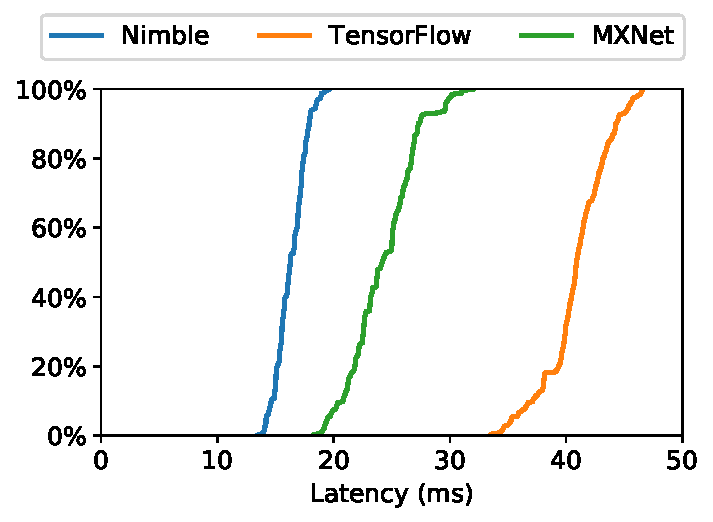
\includegraphics[height=5cm]{figs/bert_cdf_c5.pdf}
%     \caption{BERT latency CDF on Intel CPU.}
%     \label{fig:bert-cdf}
% \end{figure}

%\subsection{Optimization implications}
%\label{sec:eval:opt}
%\subsubsection{Memory planning}

%\subsubsection{Dynamic kernel dispatch}
\subsection{Microbenchmark}

% \begin{table}[t]
%     \centering
%     \begin{tabular}{c|cc|cc}
%         \toprule
%         \multirow{2}{*}{Device} & TVM & Nimble  & kernel & others  \\
%         & lat. (ms) & lat. (ms) & lat. (ms) &  (ms) \\ %&  (\%) \\
%         \midrule
%         Intel  & 19.38 & 24.32 & 21.06 & 3.26 \\% & 13.4\%
%         ARM & 223.50 & 237.41 & 228.59 & 8.82 \\%& 3.72\% \\
%         Nvidia & 5.58 & 5.86 & 5.60 & 0.26 \\%& 4.44\% \\
%         \bottomrule
%     \end{tabular}
%     \caption{BERT model latency (sequence length 128) using TVM and Nimble on different hardware.
%     {\it kernel latency} shows the latency of kernel invocation in Nimble, and {\it others} shows the extra latency introduced by other instructions.
%     }
%     \label{tab:overhead}
%     \vspace{-1em}
% \end{table}

% \hide{
% \begin{figure}[t]
%     \centering
%     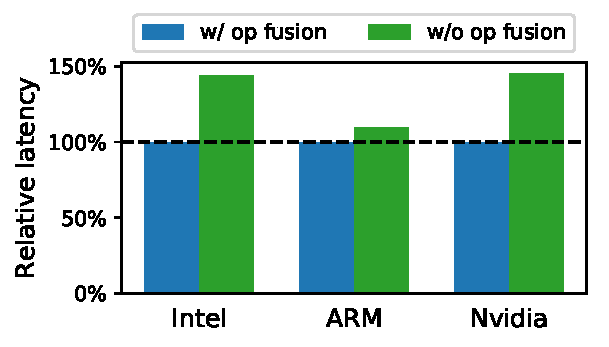
\includegraphics[height=3.5cm]{figs/op_fusion.pdf}
%     \caption{Relative latency comparison between Nimble with and without operator fusion for BERT model with sequence length 128.}
%     \label{fig:fusion}
% \vspace{-1em}
% \end{figure}
% }

\begin{figure}[t]
    \centering
    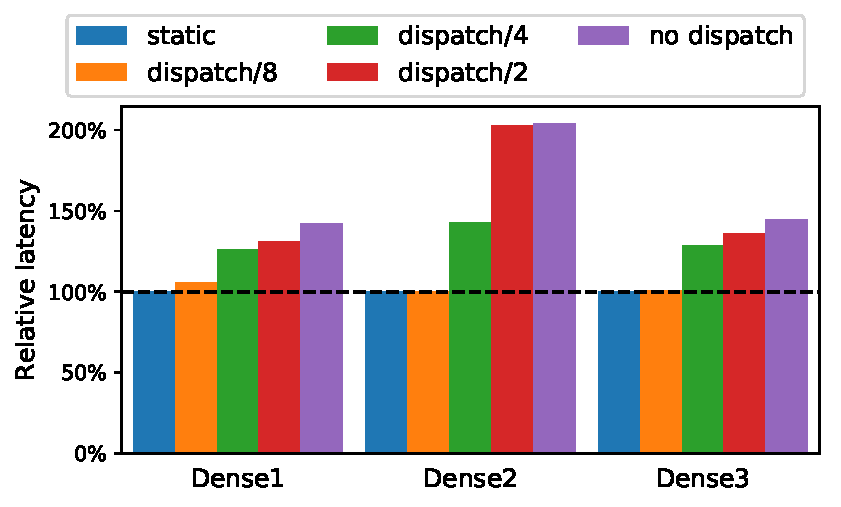
\includegraphics[height=4.5cm]{figs/sym_codegen.pdf}
    \caption{Relative latency comparison between symbolic codegen and static codegen of 3 dense operators on ARM CPU. The latency of kernel compiled with static shapes is used as the baseline. ``dispatch/$k$'' indicates that we generate $k$ symbolic kernels to be dispatched at runtime. ``no dispatch'' means that only one symbolic kernel is generated and therefore no dispatching is needed. %\protect\yida{The labels of x-axis, can we make them Dense 1, Dense 2 and Dense 3? L1, L2, L3 are like cache level to me at the first glance}
    }
    \label{fig:sym-codegen}
\end{figure}

This section analyzes the performance gain of Nimble by using BERT as the microbenchmark. Three studies will be conducted to examine (a) the overhead introduced by the VM, %(b) the effectiveness of operator fusion\yida{Can we somehow relate this to any proposed techniques? For example, op fusion is enabled by carefully taking care of shape functions?},
(b) the advantage of the proposed memory planning pass, and (c) the performance discrepancy between symbolic and static codegen.

\noindent {\bf Overhead in handling dynamism} In order to understand the overhead that Nimble spends to take care of dynamism, we compared it to TVM where static sequence length and TVM static runtime is used to execute BERT.
%\yida{how do you map this to the aforementioned four points?}
\autoref{tab:overhead} details the performance difference between Nimble and TVM.  TVM is 5\% to 25\% faster than Nimble on static shapes, though the absolute latency difference is small. The overhead comes from two aspects: (a) kernels generated with symbolic shapes cause extra overhead in the index computation. (b) other instructions in the virtual machine are required to handle the dynamic execution, such as shape functions, dynamic memory allocation, instruction dispatch, etc.
On Nvidia GPU, most of bytecode latency is overlapped with the GPU execution thanks to heterogeneous device placement (\autoref{sec:compliation:hetero}), and therefore the overhead of other instructions is negligible.

% \hide{
% \noindent {\bf Operator fusion}
% One of the most important benefits from deep learning compiler is its flexibility to fuse operators for better cache locality. \autoref{fig:fusion} depicts the comparison between Nimble with and without operator fusion. With operator fusion, the latency can be reduced by 44\%, 10\%, and 46\% on Intel CPU, ARM CPU, and Nvidia GPU, respectively. This is because operator fusion provides better opportunities for (a) achieving better cache locality, and (b) reducing the buffer allocation for temporary intermediates as well as the number of shape functions to be executed.\yida{Mention that this is not available if we don't take care of the shape functions properly. Op fusion is not our contribution, but enabling it in the context of dynamism is.}}
%so that some memory copies and synchronization between devices as well as irregular memory accesses for calculating shapes can be possibly eliminated.

\noindent {\bf Memory planning} % Memory allocation at runtime is expensive.
\autoref{sec:compliation:memory} proposed memory planning to coalesce memory allocation together and reuse the already allocated memory chunks. Thanks to this pass, we are able to reduce the number of buffer allocation by 47\%, and the memory allocation latency is reduced by 75\% from 2.0 ms to 0.5 ms on Intel CPU. We also compared the memory usage of Nimble with memory planning to TVM which statically analyze and pre-allocate memory on popular computer vision models such as ResNet~\citep{he2016deep}, MobileNet~\citep{howard2017mobilenets}, VGG~\citep{simonyan2014very} and SqueezeNet~\citep{iandola2016squeezenet}. It turned out that Nimble leads up to 8\% more memory footprint.

\noindent {\bf Symbolic codegen} We selected 3 dense operators in the BERT model and compared the performance of symbolic codegen against static codegen on ARM CPU.
%\yida{Can we claim that similar observation can be got for other platforms? State it if yes (I know that the performance is worse than libraries, but we don't need to mention this)}.
\autoref{fig:sym-codegen} illustrates the relative latency of kernels generated with symbolic shapes to the baseline -- kernel compiled with static shapes. The auto-tuning algorithm chooses to tile the symbolic dimension corresponding to the dynamic sequence length by a factor of 8 in all three kernels. We varied the number of generated kernels to be dispatched during the symbolic codegen from 8 (full dispatch) to 1 (no dispatch) as described in \autoref{sec:compliation:codegen}. We observe that symbolic codegen with full dispatch can achieve nearly identical performance as that for static shapes. While reducing the number of kernels, latency increases up to 42\%, 104\%, and 45\% for these 3 layers, respectively.
We observe similar trends in dense operators with different shapes, other operators, and other platforms as well.



% \subsubsection{Memory pass}

% \subsubsection{Symbolic code generation}

% \subsubsection{VM overhead}
% \label{sec:eval:overhead}
% Finally, we compared the performance of model inference for static neural networks using Nimble with unmodified TVM. TVM is known to be efficient in processing CNN models on various hardware platforms~\citep{tvm_osdi18, liu2019optimizing}. Nimble extended TVM to support dynamism while inheriting the optimizations original TVM has. Nimble's VM-based runtime was designed to be generic enough to handle static model inference as well. Therefore, comparing between Nimble and the original TVM on static model inference should indicate how much overhead Nimble introduces while introducing dynamic support.

% \autoref{fig:static-performance} and \autoref{fig:memory-overhead} show the latency and memory footprint comparison between Nimble and original TVM on different static CNN models. The models were optimized via the TVM pipeline in both systems. The difference is that Nimble uses its VM-based runtime while TVM uses its original graph runtime. From the figure we can tell that Nimble's VM-based runtime adds minimal overhead compared to TVM's original runtime, by adding up to 13\% more execution time and 8\% more memory footprint. Also, \autoref{fig:memory-overhead} further testifies that our memory planning optimization reduces the memory usage on static model inference as well.

% We have evidence that this overhead is due to missing micro-optimizations, and not inherent to our approach, and should be erased over time.

% \begin{figure}
% \centering
% \input{figs/static_perf}
% \caption{Latency comparison between Nimble and TVM on static model inference. The latency was tested for both systems on Intel CPUs, Nvidia GPUs and ARM CPUs by setting batch size=1. The latency of TVM on those platforms was normalized to 1, the lower the better.}
% \label{fig:static-performance}
% \end{figure}

% \begin{figure}
% \centering
% \input{figs/memory}
% \caption{Memory usage comparison between Nimble and TVM on static models. Nimble was done with and without optimization on memory planning. The results were obtained on Intel CPUs. Nvidia GPUs and ARM CPUs would lead to the identical results. The amount of memory used by TVM was normalized to 1, the lower the better.}
% \label{fig:memory-overhead}
% \end{figure}




\begin{comment}
\begin{figure*}[t]
  \centering
  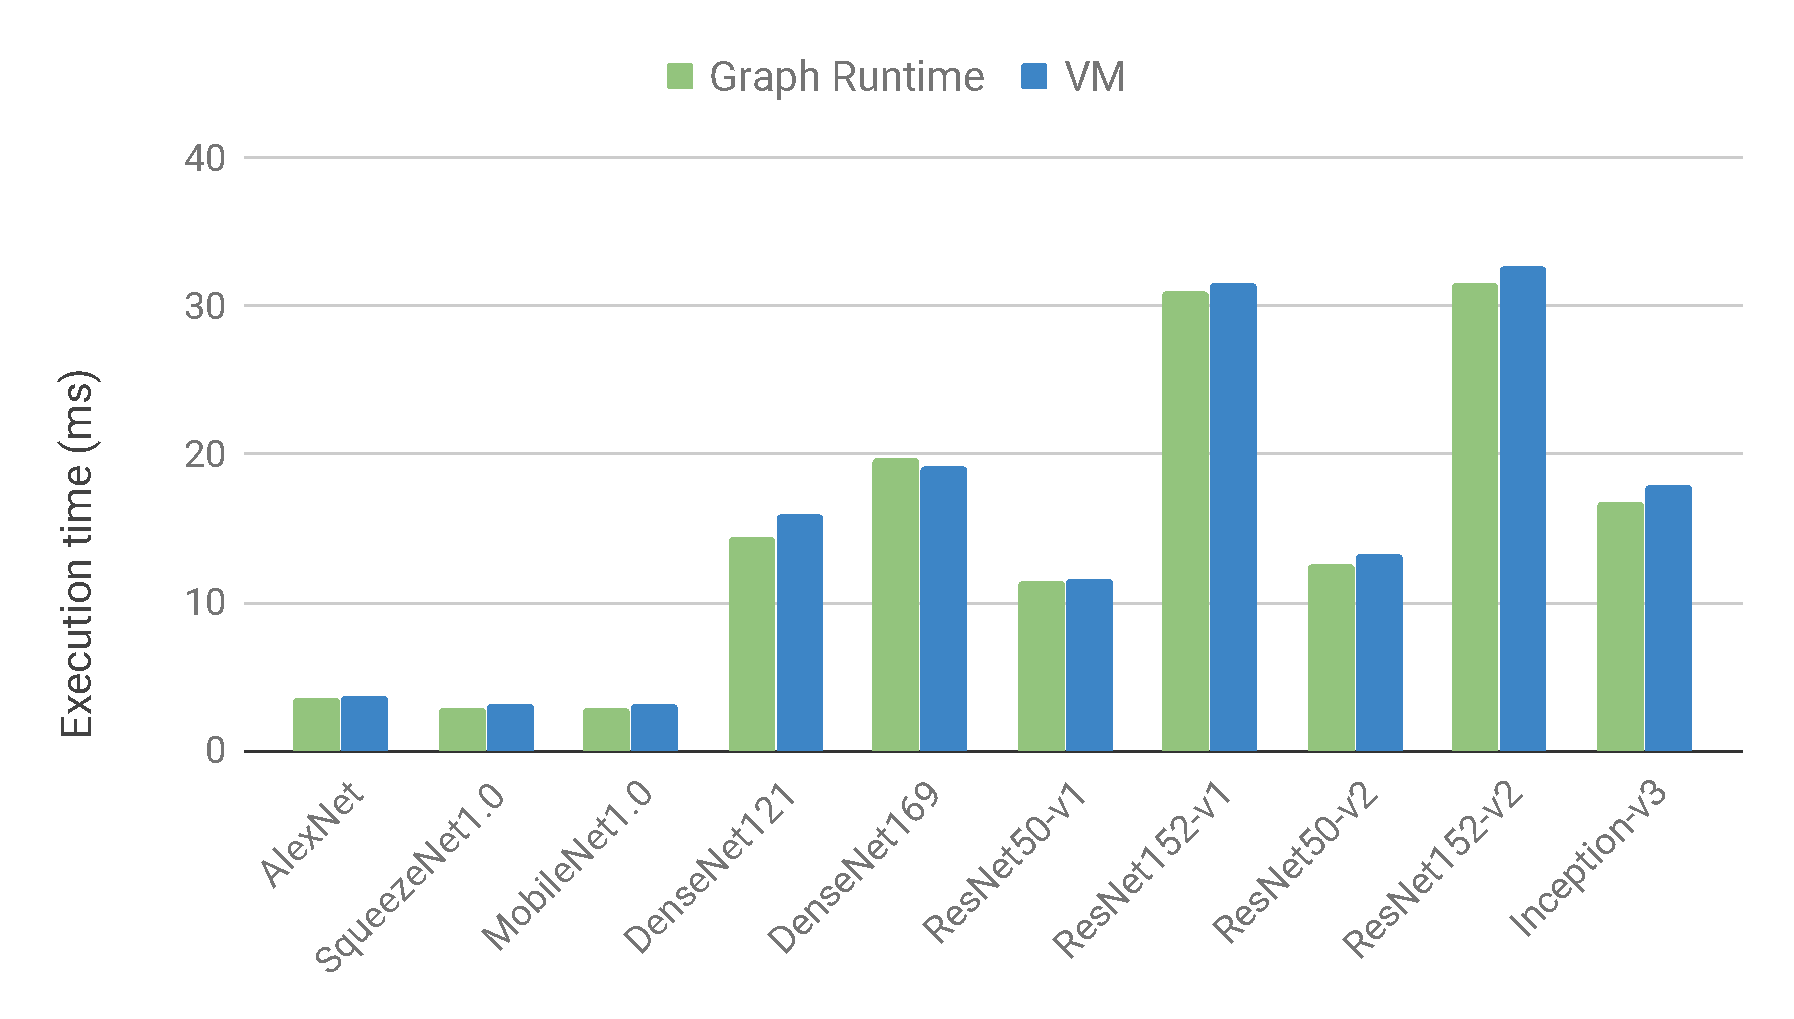
\includegraphics[width=.8\linewidth]{figs/cv_models.pdf}
  \caption{Benchmarking results of graph runtime vs. Nimble.}
  \label{fig:benchmark}
\end{figure*}

\begin{table*}[t]
\centering
\begin{tabular}{llllrrc}
\toprule
\multicolumn{1}{c}{\multirow{2}{*}{input size}} & \multicolumn{1}{c}{\multirow{2}{*}{hidden size}} & \multicolumn{1}{c}{\multirow{2}{*}{\# layers}} & \multicolumn{1}{c}{\multirow{2}{*}{seq length}} & \multicolumn{2}{c}{latency (ms)}                         & \multicolumn{1}{c}{\multirow{2}{*}{speedup ($\times$)}} \\
\multicolumn{1}{c}{}                            & \multicolumn{1}{c}{}                             & \multicolumn{1}{c}{}                          & \multicolumn{1}{c}{}                            & \multicolumn{1}{c}{MxNet} & \multicolumn{1}{c}{Relay VM} & \multicolumn{1}{c}{}                             \\
\midrule
100                                             & 100                                              & 1                                             & 1                                               & 0.53                      & 0.03                         & 18.4                                             \\
100                                             & 100                                              & 1                                             & 20                                              & 4.74                      & 0.52                         & 9.2                                              \\
100                                             & 100                                              & 1                                             & 100                                             & 21.75                     & 2.57                        & 8.5                                              \\
100                                             & 100                                              & 2                                             & 100                                             & 30.53                     & 4.79                         & 6.4                                              \\
100                                             & 100                                              & 3                                             & 100                                             & 55.47                     & 7.04                         & 7.9                                              \\
200                                             & 600                                              & 3                                             & 100                                             & 67.14                     & 35.16                        & 1.9                                              \\
400                                             & 1150                                             & 3                                             & 100                                             & 166.54                    & 123.54                       & 1.3                                              \\
1500                                            & 1500                                             & 2                                             & 100                                             & 182.71                    & 138.78                       & 1.3
\\\bottomrule
\end{tabular}
\vspace{6pt}
\caption{Compare performance of LSTM models between MxNet and Relay VM.}
\label{tab:lstm}
\end{table*}

We evaluated the model inference with the VM against the TVM graph runtime on a number of popular vision models, including AlexNet, ResNet, MobileNet, VGG, DenseNet, SqueezeNet and Inception. Models are from GluonCV model zoo.  We repeated the inference 100 times for each model, obtained the performance result by averaging the execution times. All experiments were performed on Amazon EC2 C5.9xlarge instance (Intel Skylake-SP, 72 GiB memory, 18 physical cores, featured with AVX-512). In general, VM reached comparable inference performance even some optimizations were not plugged. As shown in \autoref{fig:benchmark}, we observed VM provided 2.59\% performance improvement on DenseNet169. On the rest of models, VM introduced some performance regression. We saw 11.3\% performance drop on SqueezeNet1.0.

We also evaluated the inference performance of recurrent models, which requires control flow support. We choose LSTM model \citep{hochreiter1997long} and vary the input size, hidden size, number of layers, and sequence length. We measured the execution time of LSTM models for both MxNet MKL 1.4.1 and Relay VM on Amazon EC2 C5.9xlarge instance. \autoref{tab:lstm} shows that Relay VM can achieve 6.4-18.4$\times$ speedup on small LSTM models and 1.3-1.9$\times$ speedup on larger models.
\end{comment}
